\section{1174095 - Muhammad Dzihan Al-Banna}

\subsection{Teori}
\begin{enumerate}

        \item Jelaskan dengan ilustrasi gambar sendiri apa perbedaan antara vanilla GAN dan cGAN.
		Generator dan Disciminator pada Vanilla GAN adalah pembelajaran multi-layer yang sederhana, dimana algoritmanya sederhana yang mencoba untuk mengoptimasi persamman matematika menggunakan penurunan gradien stokastik. Sedangkan cGAN dapat dideskripsikan sebagai deep learing pada parameter kondisional diberlakukan.
			\begin{figure}[H]
            	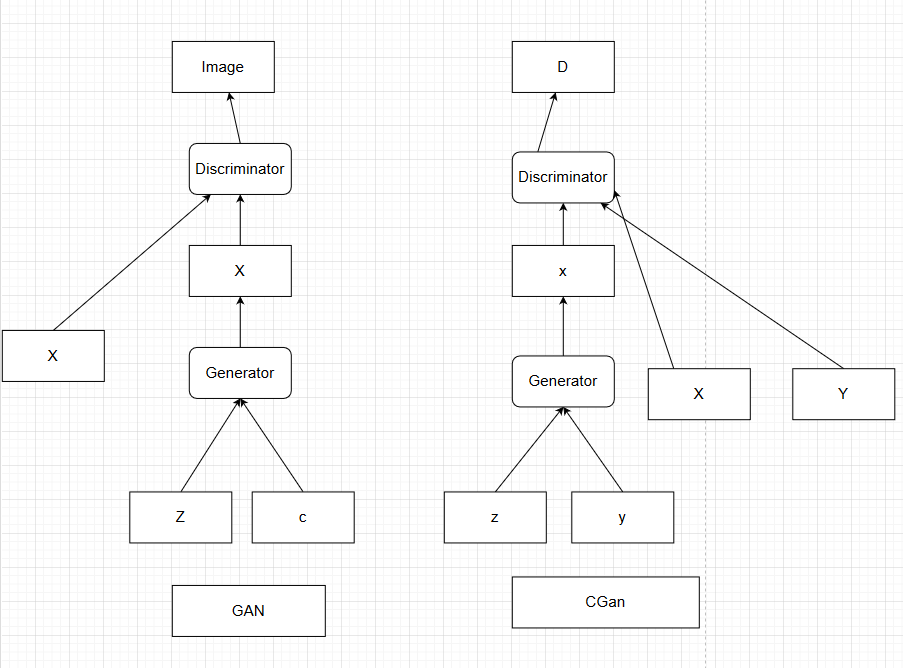
\includegraphics[width=4cm]{figures/1174095/chapter9/teori1.PNG}
           		\centering
           		\caption{Valina GAN-cGAN}
            \end{figure}
            
        \item Jelaskan dengan ilustrasi gambar sendiri arsitektur dari Age-cGAN.
		Age cGAN mempunyai 4 jaringan yang  di latih dalam 3 tahapan yaitu: Conditional GAN Training,Initial latent vector approximation,dan Latent vector optimization.
			\begin{figure}[H]
				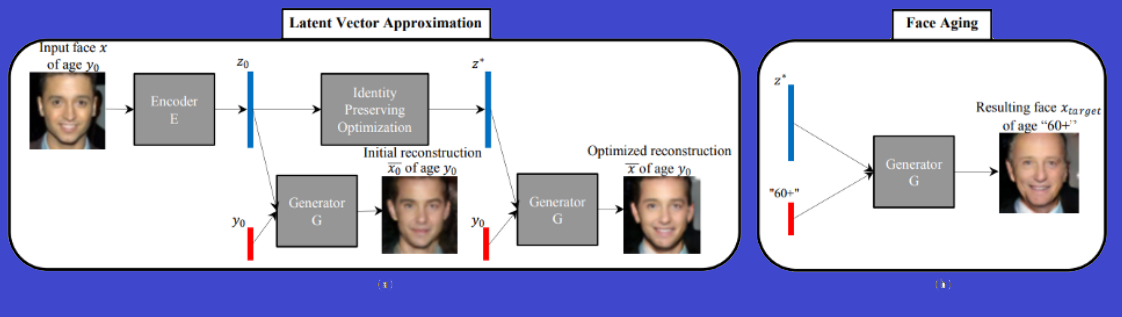
\includegraphics[width=4cm]{figures/1174095/chapter9/teori2.PNG}
            		\centering
           		\caption{Age-cGAN}
            \end{figure}
                
        \item Jelaskan dengan ilustrasi gambar sendiri arsitektur encoder network dari AgecGAN.
		Arsitektur encoder biasanya digunakan untuk mengenerate latent vector dari gambar yang akan diinputkan yang nantinya akan diteruskan ke generator.
            \begin{figure}[H]
                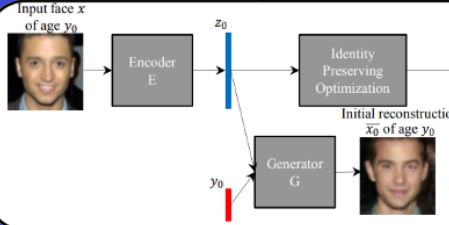
\includegraphics[width=4cm]{figures/1174095/chapter9/teori3.PNG}
                    \centering
                \caption{Encoder Age cGANr}
            \end{figure}

        \item Jelaskan dengan ilustrasi gambar sendiri arsitektur generator network dari AgecGAN.
		Arsitektur generator adalah sebuah CNN dan mengambil 100-dimensional latent vector sebagai inputannya yang akan menghasilkan gambar realistik dalam dimensi (64,64,3)
		\begin{figure}[H]
			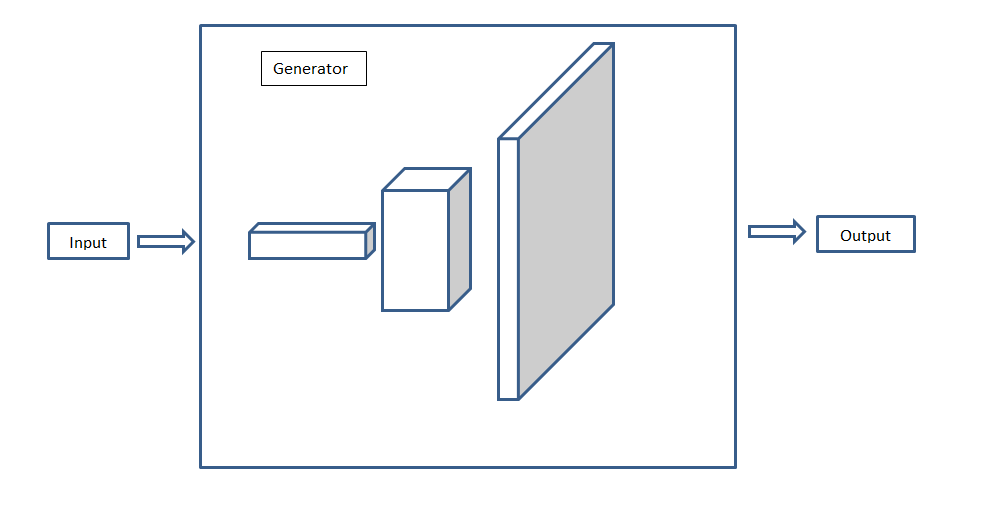
\includegraphics[width=4cm]{figures/1174095/chapter9/teori4.PNG}
            	\centering
           	\caption{Network Age cGAN}
       	\end{figure}


        \item Jelaskan dengan ilustrasi gambar sendiri arsitektur discriminator network dari Age-cGAN.
		Arsitektur diskriminator adalah CNN yang fungsinya untuk memprediksi apakah gambar yang diberikan palsu atau asli.
		\begin{figure}[H]
			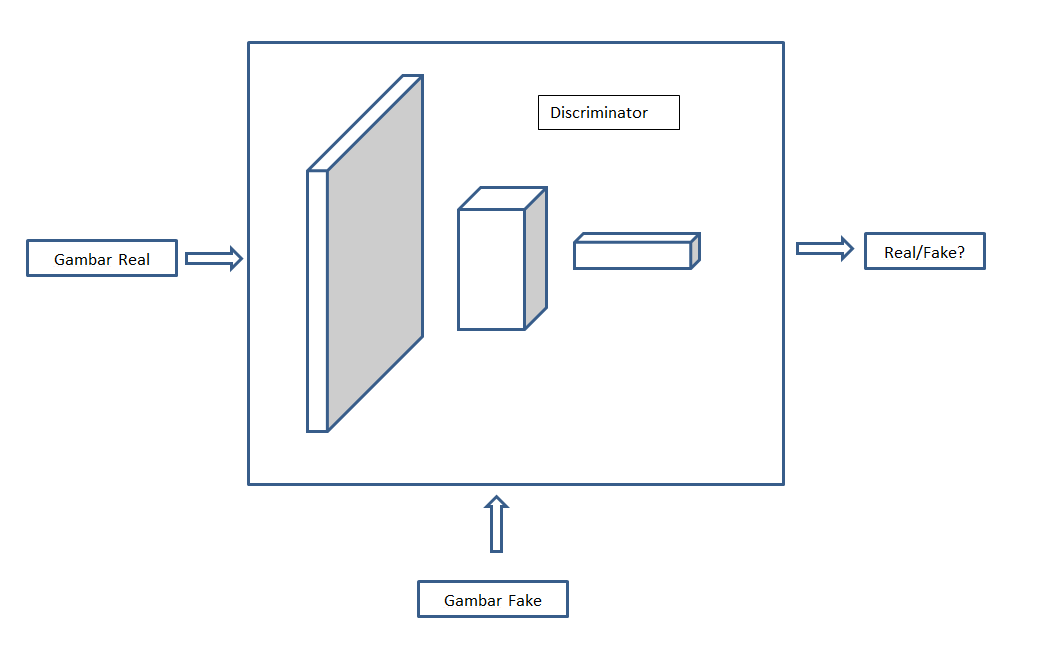
\includegraphics[width=4cm]{figures/1174095/chapter9/teori5.PNG}
            	\centering
           	\caption{Discriminator Age cGAN}
       	\end{figure}


        \item Jelaskan dengan ilustrasi gambar apa itu pre-trained Inception-ResNet-2 Model.
		Pre-Trained Network atau Transfer Learning merupakan suatu metode penyelesaian yang memanfaatkan model yang sudah dilatih terhadap suatu dataset untuk menyelesaikan masalah dengan cara menggunakan sebagai starting point, memodifikasi dan mengupdate parameternya, sehingga sesuai dengan dataset yang baru.
		\begin{figure}[H]
			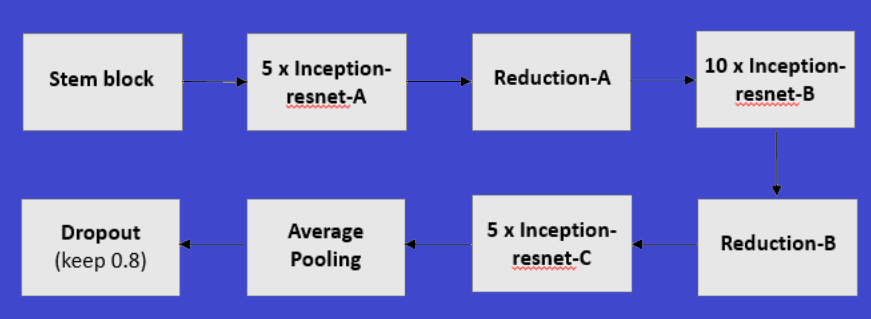
\includegraphics[width=4cm]{figures/1174095/chapter9/teori6.PNG}
            	\centering
           	\caption{Pretrained Inception ResNet}
       	\end{figure}

        \item Jelaskan dengan ilustrasi gambar sendiri arsitektur Face recognition network Age-cGAN.
		Face Recognition digunakan untuk mengenali identitas seseorang dari gambar yang diberikan.
		\begin{figure}[H]
			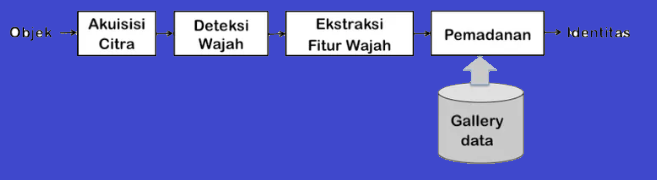
\includegraphics[width=4cm]{figures/1174095/chapter9/teori7.PNG}
            	\centering
           	 \caption{Face recognition network Age-cGAN}
       	 \end{figure}

        \item Sebutkan dan jelaskan serta di sertai contoh-contoh tahapan dari Age-cGAN.
		Pada dari Age-cGan ni terdapat 2 tahapan dengan generator dan diskriminator. dimana untuk tahap generator sendiri membutuhkan vektor laten 100 serta menghasilkan gambar yang realistis dari dimensinya. sedangkan tahap diskriminator itu tahapan dimana memprediksi gambar yang diberikan nyata atau palsu.
		\begin{figure}[H]
			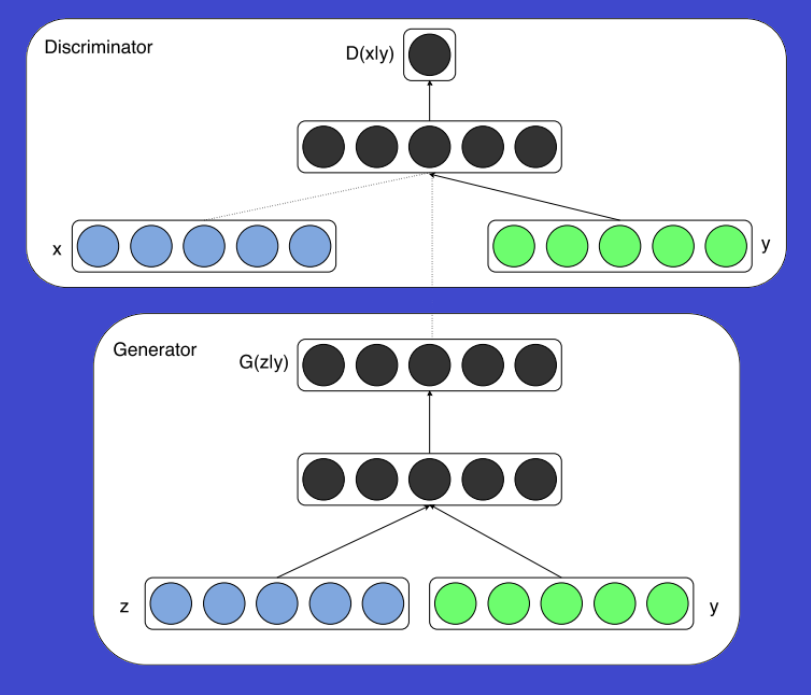
\includegraphics[width=4cm]{figures/1174095/chapter9/teori8.PNG}
            	\centering
           	 \caption{Tahap Age cGAN}
       	\end{figure}

        \item Berikan contoh perhitungan fungsi training objektif.
		Objektif Trainning ialah untuk meminimalkan loss function sebagai log likelihood function yang diberikan pada persamaan dimana D melambangkan trainning data.
		\begin{figure}[H]
			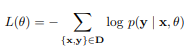
\includegraphics[width=4cm]{figures/1174095/chapter9/teori9.PNG}
            	\centering
           	 \caption{Training Objektif}
       	\end{figure}

        \item Berikan contoh dengan ilustrasi penjelasan dari Initial latent vector approximation.
		Latent vector approdimation kemampuan untuk membuat gamar yang realistis dan tajam serta menghasilkan gambar wajah pada usia target.
		\begin{figure}[H]
			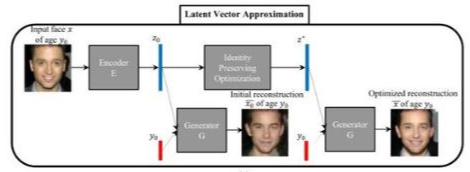
\includegraphics[width=4cm]{figures/1174095/chapter9/teori10.PNG}
            	\centering
           	 \caption{Initial Latent Vector Approximation}
       	\end{figure}

        \item Berikan contoh perhitungan latent vector optimization.
		Perhitungan lantent optimization menggunakan metode yang relatif sederhana, tergantung pada jumlah kecil parameter yang diperlukan, sehingga pada latent optimization dapat memetakan setiap gambar x dari dataset ke vektor acak dimensi rendah zi dalam ruang laten z.
		\begin{figure}[H]
			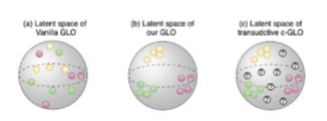
\includegraphics[width=4cm]{figures/1174095/chapter9/teori11.PNG}
            	\centering
           	\caption{Latent Vector Optimization}
        \end{figure}
           
\end{enumerate}

\subsection{Praktek}

    \begin{enumerate}
	\item Jelaskan bagaimana cara ekstrak file dataset Age-cGAN menggunakan google colab.
    Kode dibawah ini digunakan untuk membuat notebooks baru, kemudian membuat ekstraksi file dari link dataset.
	\lstinputlisting[firstline=1, lastline=4]{src/1174095/chapter9/chap9.py}

	\item Jelaskan bagaimana kode program bekerja untuk melakukan load terhadap dataset yang sudah di ekstrak, termasuk bagaimana penjelasan kode program perhitungan usia.
    Kode dibawah berfungsi untuk melakukan fungsi perhitungan usia.
	\lstinputlisting[firstline=6, lastline=31]{src/1174095/chapter9/chap9.py}

	\item Jelaskan bagaimana kode program The Encoder Network bekerja dijelaskan dengan bahawa awam dengan ilustrasi sederhana.
    Berikut adalah proses Encoder dengan vector latent Z yang berfungsi untuk mempelajari pemetaan terbalik dari gambar wajah dan kondisi usia .
	\lstinputlisting[firstline=33, lastline=73]{src/1174095/chapter9/chap9.py}

	\item Jelaskan bagaimana kode program The Generator Network bekerja dijelaskan dengan bahawa awam dengan ilustrasi sederhana.
    Proses Generator agar bekerja dengan baik dibutuhkan representasi dari gambar wajah dan vector kondisi sebagai inputan yang menghasilkan sebuah gambar.
	\lstinputlisting[firstline=75, lastline=104]{src/1174095/chapter9/chap9.py}

    \item Jelaskan bagaimana kode program The Discriminator Network bekerja dijelaskan dengan bahawa awam dengan ilustrasi sederhana.
    Berikut adalah proses Discriminator yang digunakan untuk membedakan antara gambar asli ataupun gambar palsu yang dihasilkan oleh generator.
	\lstinputlisting[firstline=116, lastline=148]{src/1174095/chapter9/chap9.py}

    \item Jelaskan bagaimana kode program Training cGAN bekerja dijelaskan dengan bahawa awam dengan ilustrasi sederhana.
    Proses Training cGAN ini dengan load file .mat pada dataset lalu epoch sebanuak 500 kali.

	\lstinputlisting[firstline=150, lastline=167]{src/1174095/chapter9/chap9.py}

    \item Jelaskan bagaimana kode program Initial dan latent vector approximation bekerja dijelaskan dengan bahawa awam dengan ilustrasi sederhana.
    Initial dan Latent Vector Approximation bekerja melakukan predicsi epoch yang telah di buat sebanyak 500 kali, dan nanti hasilnya ada di folder result.

	\lstinputlisting[firstline=169, lastline=217]{src/1174095/chapter9/chap9.py}

\end{enumerate}

\subsection{Penanganan Error}
\begin{enumerate}
	\item Tidak ada error yang terjadi
\end{enumerate}

\subsection{Bukti Tidak Plagiat}
\begin{figure}[H]
	\centering
		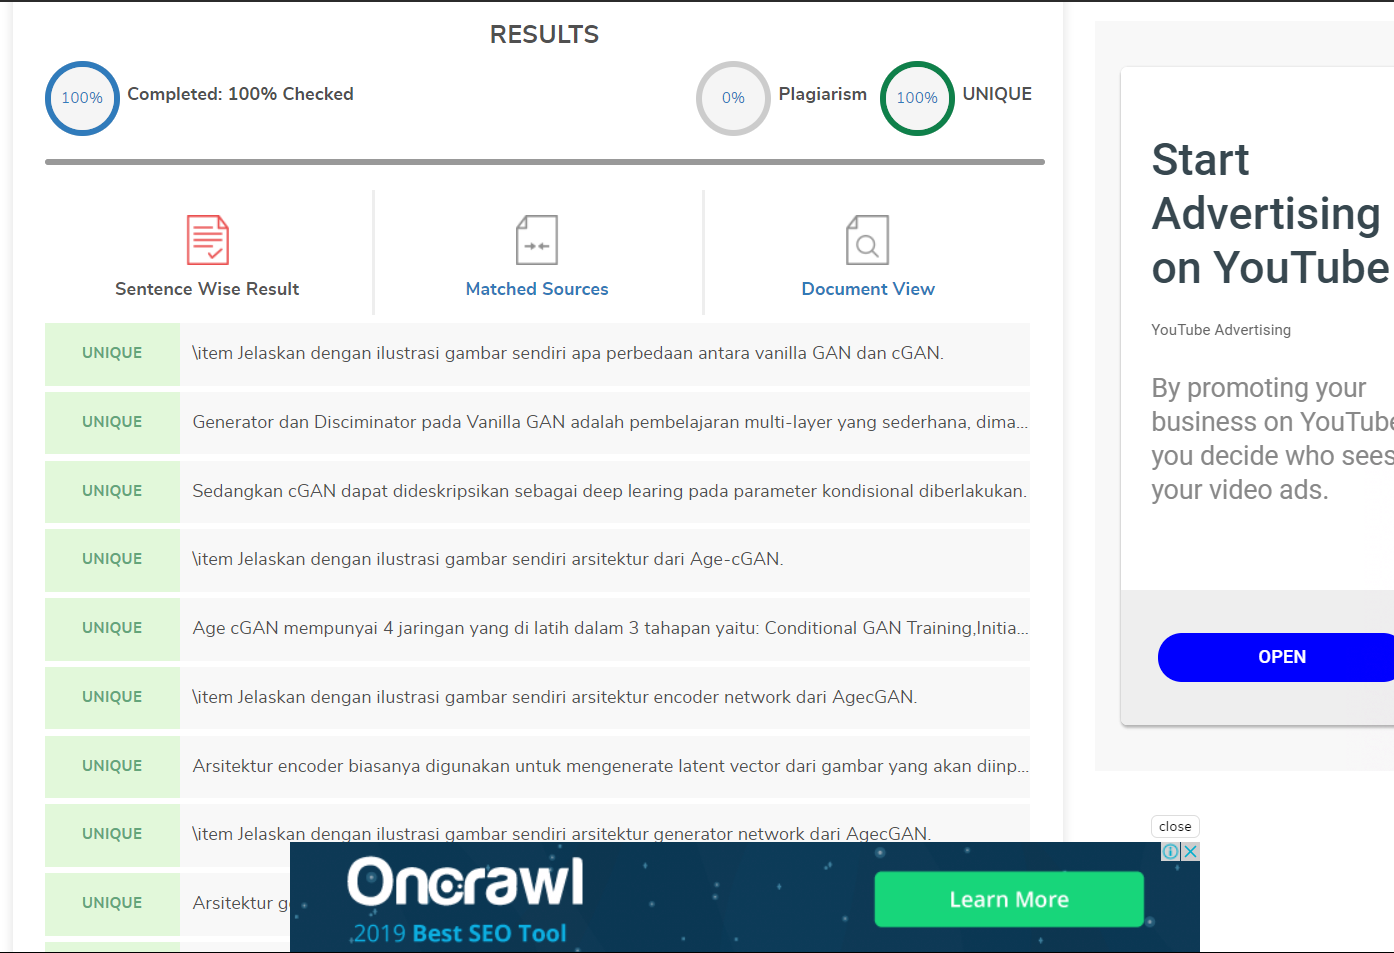
\includegraphics[width=4cm]{figures/1174095/chapter9/plagiaris.PNG}
		\caption{Bukti Tidak Melakukan Plagiat Chapter 9}
	\end{figure}

